\documentclass[11pt,a4paper]{article}
\usepackage[a4paper,margin=2.25cm]{geometry}
\usepackage{amsmath,amssymb,amsthm,booktabs,graphicx,float,array}
\usepackage[numbers]{natbib}
\usepackage{xcolor,hyperref,microtype,enumitem,caption,placeins}
\hypersetup{colorlinks=true,linkcolor=teal,citecolor=teal,urlcolor=teal}
\captionsetup{font=small,skip=5pt}
\setlength{\emergencystretch}{3em}
\newtheorem{proposition}{Proposition}
\newcommand{\E}{\mathbb{E}}
\newcommand{\Aset}{\mathcal{A}}
\newcommand{\Pset}{\mathcal{P}}
\newcommand{\datafolder}{artifacts/user_provider_game/20260906/}
\graphicspath{{figures/user_provider_game_20260906/}}
\makeatletter
\newcommand{\inputtable}[1]{\@@input #1 }
\makeatother

\title{Strategic User Timing under Competing LLM Service Prices:\\An Atomic Congestion Game with Explicit Before--After Comparisons}
\author{Research manuscript}
\date{6 September 2026}

\begin{document}
\maketitle
\begin{abstract}
Time-varying inference prices can encourage users to defer flexible work, but a stable user response need not improve welfare relative to another tariff. We formulate a two-stage game in which two manufacturers commit to price schedules and atomic request agents choose a provider and a feasible execution period. User utility subtracts the bill, delay cost, switching cost, and load-dependent quality loss from task value. Equal normalized workloads and a shared congestion penalty give the user subgame an exact potential. Strict best responses terminate at an individually stable assignment; the manufacturers compete over a declared finite price menu, anticipating the selected user equilibrium after every price pair. In a workload-shape-anchored synthetic cohort of 240 agents, user responses to the same final time-of-use prices reduce mean bills by 6.52\%, generalized costs by 4.68\%, and expected peak load by 10.07\%. Mean utility rises by 0.0502 normalized units, although 49.58\% of agents have lower final expected utility. This within-price result does not establish tariff superiority: compared with a uniform-price equilibrium with equally strategic users, time-of-use pricing raises mean bills by 13.66\% and reduces mean utility by 0.1237 units. The adverse utility difference persists in five predefined cohorts. A replay of all 50,625 distinct scenario--price combinations verifies user deviations and manufacturer payoff matrices with independently implemented utility and accounting equations. The evidence establishes finite-game stability and a clear adaptation effect, not a continuous-price equilibrium, empirical market validation, or a welfare guarantee.
\end{abstract}

\section{Introduction}
Users invoke LLM services through coding, dialogue, writing, and data-analysis interfaces. Some requests need an immediate response; others can wait until a declared deadline. A price-aware user may therefore change both the provider and the execution time. These are personal decisions: a user accepts delay only when the resulting bill and service quality justify its cost under the stated utility model. Manufacturers, meanwhile, select prices to increase their own profits. The two objectives need not agree.

An explicit user game is needed to distinguish voluntary response from an aggregate demand-allocation rule. A schedule can look smooth while leaving some users with profitable deviations. Conversely, an assignment can be stable for every user while producing a lower average utility than another pricing regime. We study both issues by separating three questions: whether users improve their average outcome by responding to a fixed tariff, whether the final assignment is individually stable, and whether competing time-of-use tariffs outperform competing uniform tariffs for those users.

The contribution is a verifiable model and comparison protocol, not a new general equilibrium theorem. We combine bounded release--deadline choices with atomic provider congestion, compute the selected user equilibrium for every manufacturer price pair, and keep within-price adaptation separate from cross-tariff welfare. The positive before--after effect and the negative tariff comparison are both substantive results. Neither is discarded to make the proposed interaction appear uniformly beneficial.

\section{Context and Scope}
LLM pricing research already links provider prices with user service choices. PriLLM models data-calibrated Stackelberg pricing and routing with user preferences and quality considerations \cite{guo2026prillm}. Our model isolates a narrower question: how explicit release--deadline timing choices interact with provider competition in a finite, inspectable user congestion game. We do not claim that this model subsumes the online routing or scaling objectives of prior work.

The user layer follows the congestion-game tradition of Rosenthal \cite{rosenthal1973class}. Its exact potential is available because every task contributes one unit to one provider--period resource and all agents share the same congestion penalty for that resource. User-specific delay and switching terms enter additively. The manufacturer layer is a finite bimatrix game, for which mixed Nash equilibria exist \cite{nash1951noncooperative}. These foundations do not guarantee that a particular numerical output is accurate; the implementation must still check all unilateral deviations on the declared strategy sets.

BurstGPT supplies an observed intraday workload shape \cite{wang2025burstgpt}, not observed price responses. Application marks in Fig.~\ref{fig:framework} identify possible interfaces, not distinct calibrated populations. The primary experiment has two direct-access manufacturers. An API intermediary, heterogeneous model capabilities, user exit, and online arrival uncertainty are outside this model. Older aggregate-choice experiments are preserved separately; their numerical results and equilibrium claims are not reused here.

\begin{figure}[htbp]
\centering
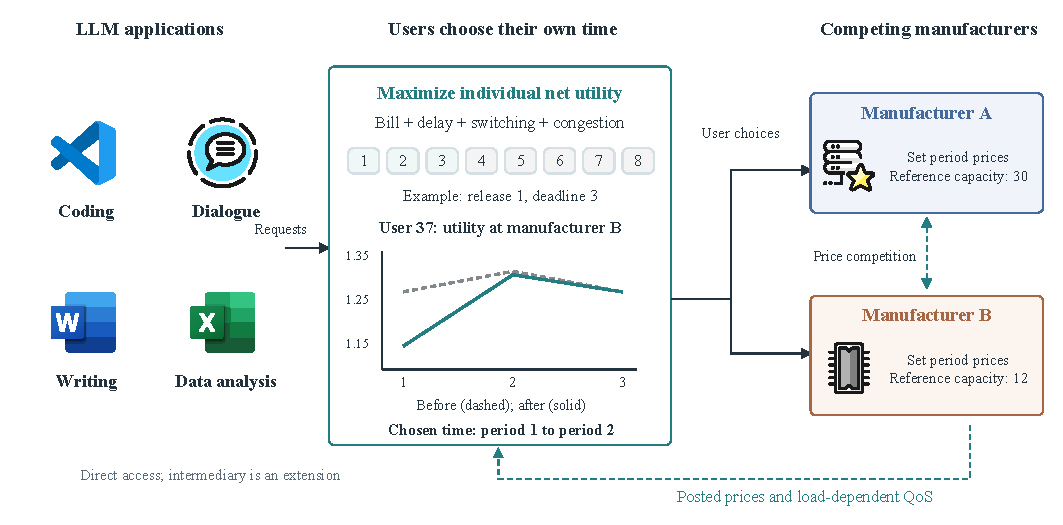
\includegraphics[width=\textwidth]{user_game_framework.pdf}
\caption{Applications, individual time choice, and competing manufacturers. Users minimize their own combined bill, delay, switching, and congestion costs after prices are announced. The center inset uses the actual prospective utilities of user 37 at manufacturer B, at the representative price pair; it is not a hand-drawn gain curve. This user is the smallest-index actual time switcher, a post-hoc mechanism illustration without a utility-gain filter. The predeclared first flexible user is retained in Fig.~\ref{fig:users}. Solid arrows show choices and dashed arrows information or competition. Service and dialogue pictograms are by Streamline (CC BY 4.0); application marks are sourced from vscode-icons with original owners' rights retained. No endorsement is implied.}
\label{fig:framework}
\end{figure}

\section{User--Manufacturer Game}
\subsection{Timing and feasible user actions}
Two manufacturers $m\in\{A,B\}$ simultaneously commit to complete daily price schedules $p_m$. After observing the realized pair $p=(p_A,p_B)$, $N$ request agents choose their provider and execution period. Manufacturer randomization, when needed, occurs before the user subgame. Users respond to the realized schedule, not to the average of several schedules.

A day contains $T$ periods of length $h$ hours. Agent $i$ has release period $r_i$, deadline $d_i$, and preferred manufacturer $b_i$. Its action set is
\begin{equation}
 \Aset_i=\{(m,t):m\in\{A,B\},\ r_i\leq t\leq d_i\}.
\end{equation}
Time-rigid agents have $d_i=r_i$ but may still change manufacturer. Flexible agents may defer, never execute before release, and never wrap around the day boundary. The initial assignment is $a_i^0=(b_i,r_i)$. Every agent has one normalized task and must select exactly one feasible action. Thus total load is conserved; there is no cancellation or outside option.

For assignment $a$, let $n_{mt}(a)=\sum_i\mathbf{1}\{a_i=(m,t)\}$. Manufacturer capacity $K_m$ is a per-period reference load. It is not a hard feasibility constraint. Overload affects a quality proxy
\begin{equation}
 q_m(n)=\exp\left[-\eta\left(\max\left\{n/K_m-\theta,0\right\}\right)^2\right].
 \label{eq:qos}
\end{equation}
The deadline restricts the selected period only; the model does not simulate a queue or guarantee physical completion before the deadline.

\subsection{Individual utility and prospective congestion}
For $a_i=(m,t)$, utility is
\begin{equation}
 U_i(a;p)=v_i-p_{mt}-\delta_i h(t-r_i)-\kappa\mathbf{1}\{m\ne b_i\}
          -g_m(n_{mt}(a)),\qquad g_m(n)=\gamma[1-q_m(n)].
 \label{eq:utility}
\end{equation}
Here $v_i$ is task value, $\delta_i$ is delay cost per hour, $\kappa$ is the manufacturer-switching cost, and $\gamma$ monetizes the shared quality loss. The generalized cost is $C_i=v_i-U_i$. Bills are the posted prices; quality does not discount payments in this model.

The relevant deviation is evaluated \emph{after} the user's own task joins its destination. For candidate $s=(m,t)$, the prospective load is
\begin{equation}
 n_s^{(i)}=n_s(a)+1-\mathbf{1}\{a_i=s\}.
 \label{eq:ownload}
\end{equation}
Omitting the added unit would give an incorrect incentive near capacity. A user best response minimizes $p_{mt}+\delta_i h(t-r_i)+\kappa\mathbf{1}\{m\ne b_i\}+g_m(n_s^{(i)})$ over $\Aset_i$. The maximum remaining utility improvement is
\begin{equation}
 R_U(a;p)=\max_i\max_{s\in\Aset_i}\big[U_i(s,a_{-i};p)-U_i(a;p)\big]_+.
 \label{eq:userregret}
\end{equation}
We certify the computed user assignment when $R_U\leq10^{-8}$. This is conditional individual optimality given other users' final actions and the realized prices. It is not maximization of a common welfare objective.

\subsection{Manufacturer prices and profits}
The exogenous normalized native-load signal $z_t$ has zero unweighted mean and $\max_t|z_t|=1$. Manufacturer $m$ chooses a schedule from a finite menu:
\begin{equation}
 p_{mt}=\beta_m+\alpha_m z_t,\qquad
 \beta_m\in[0.45,1.05],\quad \alpha_m\in[-0.30,0.30].
 \label{eq:tariff}
\end{equation}
Every posted price must lie in $[0.30,1.35]$. Invalid schedules are discarded rather than clipped, so the mean price remains $\beta_m$. The uniform regime permits only $\alpha_m=0$; time-of-use (TOU) pricing permits both signs. These are precommitted period prices, not an online feedback or reinforcement-learning policy.

Let $F(p)$ denote the user equilibrium selected by the fixed initialization, fixed response order, and tie rule in Section~\ref{sec:algorithm}. Manufacturer profit is
\begin{equation}
 \Pi_m(p)=\sum_t(p_{mt}-c_m)n_{mt}(F(p))-fTK_m,
 \label{eq:profit}
\end{equation}
where $c_m$ is the per-task operating cost and $f$ is the per-period capacity holding cost. Counts are per-period task quantities, not hourly rates, so revenue is not multiplied by $h$. Each billed task is assigned to exactly one manufacturer, giving $\sum_i p_{a_i}=\sum_{m,t}p_{mt}n_{mt}$.

For finite menus of size $L$, define matrices $A_{jk}=\Pi_A(p_A^j,p_B^k)$ and $B_{jk}=\Pi_B(p_A^j,p_B^k)$. For manufacturer mixtures $x,y$, the full-menu regrets are
\begin{align}
 R_A&=\max_j(Ay)_j-x^\top Ay, &
 R_B&=\max_k(x^\top B)_k-x^\top By.
 \label{eq:providerregret}
\end{align}
They must not exceed $10^{-7}$. Manufacturer deviations allow users to re-equilibrate through $F$; user deviations hold prices fixed. These are different unilateral-deviation tests.

\section{Algorithm and Guarantees}\label{sec:algorithm}
\subsection{Exact potential of the user subgame}
Let $w_i(m,t)=p_{mt}+\delta_i h(t-r_i)+\kappa\mathbf{1}\{m\ne b_i\}$. The following potential applies for fixed prices:
\begin{equation}
 \Phi(a;p)=\sum_i w_i(a_i)+\sum_{m,t}\sum_{k=1}^{n_{mt}(a)}g_m(k).
 \label{eq:potential}
\end{equation}
\begin{proposition}
For any unilateral feasible move by agent $i$, $\Delta\Phi=\Delta C_i=-\Delta U_i$. Therefore every strict utility-improving move decreases $\Phi$, and exact strict best responses terminate at a pure user Nash equilibrium in this finite game.
\end{proposition}
\begin{proof}
If the agent moves from resource $s$ to distinct resource $s'$, only its private cost term and the two resource sums change. Removing the last term $g_s(n_s)$ and adding $g_{s'}(n_{s'}+1)$ gives
\[
 \Delta\Phi=w_i(s')-w_i(s)+g_{s'}(n_{s'}+1)-g_s(n_s)=\Delta C_i.
\]
A strict improvement cannot revisit an assignment with the same potential. The feasible assignment set is finite, so a sequence of exact strict improvements terminates. At termination there is no profitable unilateral deviation.
\end{proof}

The proof does not apply unchanged to arbitrarily weighted jobs or heterogeneous congestion multipliers. It also does not imply that $\sum_i U_i$ increases after each move. A mover improves its own utility at the time of its decision but changes congestion faced by others. Even the mover's final utility may later fall below its initial utility.

\subsection{Implemented two-stage solution}
\begin{table}[htbp]
\centering
\caption{Equilibrium computation and separate numerical certificates.}
\label{tab:algorithm}
\begin{tabular}{@{}p{.08\textwidth}p{.87\textwidth}@{}}
\toprule
Step & Operation \\
\midrule
1 & For each declared price pair, reset every agent to its preferred manufacturer at release. Use the same predeclared agent order for every pair. \\
2 & Visit agents sequentially. Evaluate every feasible provider--time action with Eq.~(\ref{eq:ownload}). Move only when cost decreases by more than $10^{-10}$; ties keep the current action. \\
3 & Repeat full sweeps until a sweep has no moves. Independently check all feasible user deviations and the potential-change identity. Reject an output with $R_U>10^{-8}$ or a potential identity error above $10^{-7}$. The implementation caps computation at 500 sweeps and rejects any uncertified result. \\
4 & Populate both manufacturer payoff matrices from the selected user responses, including price pairs outside equilibrium support. Solve the finite bimatrix game. Select the lexicographically first pure equilibrium when one exists, otherwise a returned mixed candidate with the smallest verified regret. \\
5 & Check every manufacturer action using Eq.~(\ref{eq:providerregret}). Report exact support-weighted outcomes, then replay all price pairs using independent utility, load, accounting, and user-deviation equations. \\
\bottomrule
\end{tabular}
\end{table}

One sweep costs $O(NT)$ for two manufacturers after tabulating private and resource costs. Building a menu's matrices requires $L^2$ user solves, each with its own convergence check. This is an offline finite-game calculation, not a claim of real-time scalability. The original full experiment took 209.70 seconds with four worker processes; the independent replay took 43.50 seconds in the recorded environment. These are reproducibility observations, not a performance benchmark.

\begin{proposition}
If $F(p)$ is a user Nash equilibrium for every declared price pair and $(x,y)$ is a Nash equilibrium of the induced manufacturer game, then $(x,y,F)$ specifies a subgame-perfect equilibrium of the stated two-stage finite game. With numerical tolerances, it specifies the corresponding approximately stable strategy profile.
\end{proposition}
\begin{proof}
After any realized price history, the prescribed user play is a Nash equilibrium of that continuation game. At the first stage, the manufacturer payoff matrices include the prescribed continuation after every unilateral price deviation. The manufacturer Nash conditions therefore exclude profitable first-stage deviations on the declared menus. These conditions cover all proper continuation subgames and the initial stage.
\end{proof}

We use ``manufacturer Nash competition with user Nash subgames'' to avoid suggesting simultaneous one-shot decisions by all parties. The result is conditional on the announced equilibrium selection $F$. It is not a continuous-price theorem or a guarantee against coordinated user deviations.

\section{Experimental Protocol}
The protocol was recorded before the new experiments. We generate $N=240$ equal-workload request agents and $T=8$ three-hour periods. Release times are sampled from the pinned BurstGPT mean token-load shares after normalization. Because the units are normalized tasks, this use of token shares anchors only temporal shape. We do not equate a simulated agent with a measured human or preserve the trace's heterogeneous request sizes.

Preferred manufacturers are sampled in proportion to capacities $(K_A,K_B)=(30,12)$. The baseline flexible share is 0.5, with deadlines $d_i=\min(r_i+2,T)$ for flexible agents and $d_i=r_i$ otherwise. Thus a flexible label need not imply positive slack at the end of the day. Delay costs are drawn uniformly from $[0.01,0.03]$ per hour. The same random ranking defines flexible subsets in the share controls; release, preference, delay cost, and user order are otherwise retained within a cohort.

We set $(c_A,c_B)=(0.20,0.18)$, $f=0.015$, $\kappa=0.03$, $v_i=2$, and $\gamma=2$. Only utility differences are meaningful with respect to the arbitrary value offset $v_i$. We therefore report absolute utility changes and percentage changes in generalized costs or bills, never percentage ``utility improvements.'' The quality proxy uses the existing pooled fit, $\theta\simeq1$ and $\eta=0.574708$, with RMSE 0.0561. The underlying anchor measures a 0.5-second time-to-first-token SLA rate for two Qwen2.5 model sizes on one RTX 4090, with five repeats per concurrency. Transferring this curve to normalized task loads is a modeling assumption, not a validated market demand model.

Three nested grids have 3, 5, and 9 points per parameter axis. After bounds checks, the uniform/TOU menu sizes are 3/7, 5/23, and 9/75. The main results use the finest menu. Boundary cases change the flexible share to 0.25 or 0.75, shorten the deferral window to one period, or remove time flexibility. The baseline seed is 20260906; four additional seeds through 20260910 provide five matched synthetic cohorts. Parameters are not retuned after observing the outcomes.

\subsection{What ``before'' and ``after'' mean}
\begin{enumerate}[leftmargin=*]
\item \textbf{Same-price algorithm comparison.} Draw prices from the final TOU manufacturer mixture. Compare the initial assignment $a^0$ with $F(p)$ at that exact pair. Average both over the same price-pair weights. Only user adaptation changes; the initial schedule is not an equilibrium. This is a controlled computational counterfactual, not an observed deployment experiment.
\item \textbf{Fair tariff comparison.} Compare the uniform-price equilibrium and TOU-price equilibrium. Both use fully responding strategic users and re-solved manufacturer competition. Neither regime gets a weaker follower baseline.
\item \textbf{Fixed-mean control.} Fix each manufacturer's unweighted daily mean at 0.75 and compare zero slope with slope competition. This is a restricted price game, not the main equilibrium and not a bill-neutral intervention.
\end{enumerate}
Unless a figure says ``representative,'' reported quantities are exact expectations over $x_jy_k$. In particular, peak load is $\E[\max_t\sum_m n_{mt}]$, not $\max_t\E[\sum_m n_{mt}]$. Expected minimum quality and expected maximum user regret are defined in the same order. Per-user benefit fractions compare expected utilities, not the probability that a randomly realized user--price pair benefits. No sampling error bars are attached to exact finite-support expectations.

\section{Results}
\subsection{Clear adaptation gains at the same prices}
Figure~\ref{fig:beforeafter} and Table~\ref{tab:main} provide the requested before--after comparison. With the final TOU price mixture held fixed, mean utility rises from 0.9270 to 0.9772. Mean bills fall from 0.9913 to 0.9266 (6.52\%), and generalized costs fall from 1.0730 to 1.0228 (4.68\%). Expected peak load decreases from 59.00 to 53.06 (10.07\%). The 240 tasks remain in the system, so the lower peak is not caused by demand loss.

The net utility gain can be traced to its components. Mean bill savings are 0.06466, mean delay cost rises by 0.00909, and mean switching cost rises by 0.00611. Congestion cost falls by only 0.00075. These components sum to the 0.05021 gain. Average QoS changes only from 0.9591 to 0.9595; it should not be described as a large general quality improvement. Expected minimum user QoS improves more, from 0.7746 to 0.8893.

\begin{figure}[htbp]
\centering
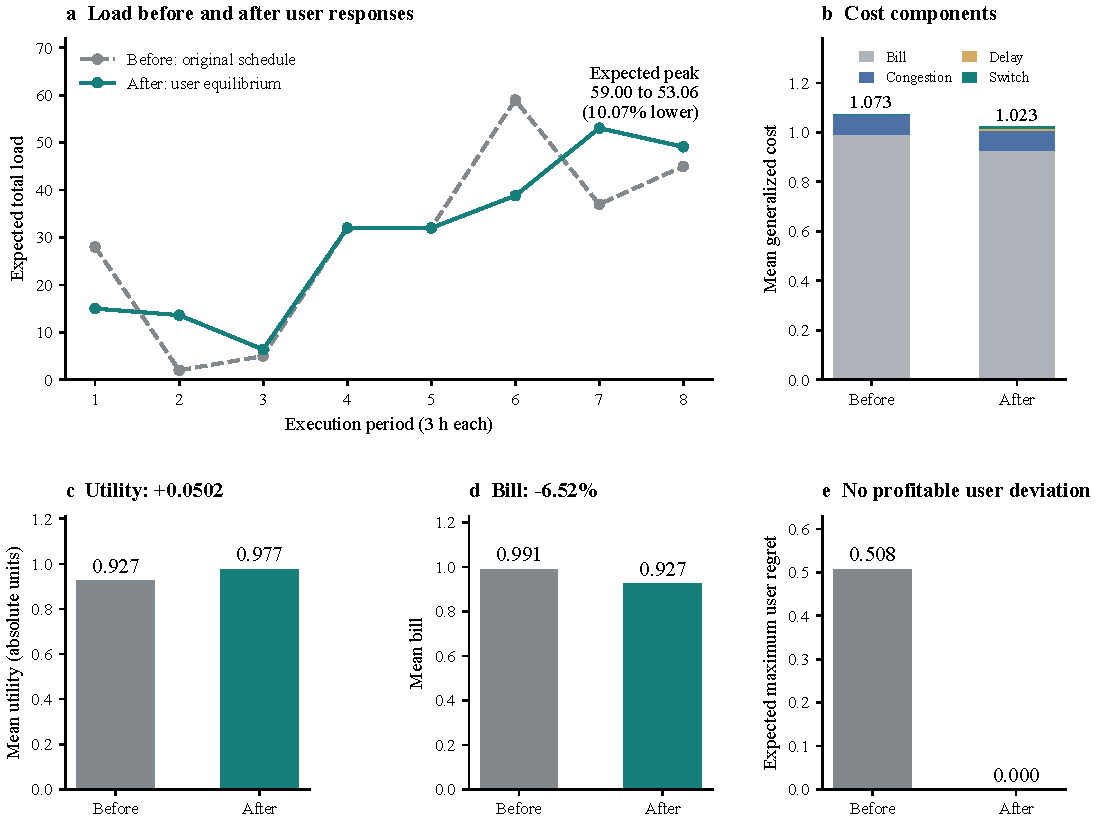
\includegraphics[width=\textwidth]{same_price_before_after.pdf}
\caption{Same final TOU prices, before and after user best responses. The cohort, feasible windows, prices, and price-pair probabilities are identical on both sides. (a) Expected period loads; the annotation reports expected maximum load. (b) Mean generalized cost components. (c) Absolute mean utility. (d) Mean bill. (e) Expected maximum user deviation gain. Before is the original schedule, not a user equilibrium. All after-price subgames have zero checked user regret, not merely a small average regret.}
\label{fig:beforeafter}
\end{figure}

The expected fraction changing time is 14.34\%, whereas 20.37\% change manufacturer; these groups may overlap. Delay averages 0.484 hours across all agents and 0.967 hours among those labeled flexible. The algorithm therefore realizes both temporal and provider substitution, and the bill benefit cannot be attributed to time shifting alone. Manufacturer A's profit falls under this fixed-price adaptation while B's rises; total profit falls from 186.20 to 171.38. The initial profit is a counterfactual under unadapted users, not a competing manufacturer equilibrium.

\begin{table}[htbp]
\centering
\caption{Matched outcome levels. TOU before/after isolates user adaptation. Uniform equilibrium/TOU after compares tariffs with equally strategic users. All costs, bills, utilities, and profits are in normalized monetary units.}
\label{tab:main}
\small
\begin{tabular}{@{}lrrr@{}}
\toprule
Metric & TOU before & TOU after & Uniform equilibrium \\
\midrule
\inputtable{artifacts/user_provider_game/20260906/main_table.tex}
\bottomrule
\end{tabular}
\end{table}

\subsection{Stable choices are not a guarantee that every user gains}
At the same prices, 121 of 240 agents (50.42\%) have higher final expected utility and 119 (49.58\%) have lower final expected utility. There are no unchanged agents at a $10^{-8}$ comparison tolerance. This does not contradict the best-response guarantee: other users alter the congestion environment after each individual move.

Figure~\ref{fig:users} preserves the predeclared first agent with positive time slack, user 0. At the representative highest-probability TOU price pair, this agent stays at manufacturer A in period 7 but its utility drops from 0.8350 to 0.7895 as other agents relocate. The final action is still a best response. For a direct illustration of actual deferral, the same figure adds user 37, the smallest-ID time switcher, without filtering on utility gain. It stays with B but moves from period 1 to 2, with realized utility rising from 1.2680 to 1.3070. The two examples do not replace the all-agent distribution in Fig.~\ref{fig:tariffs}.

\begin{figure}[htbp]
\centering
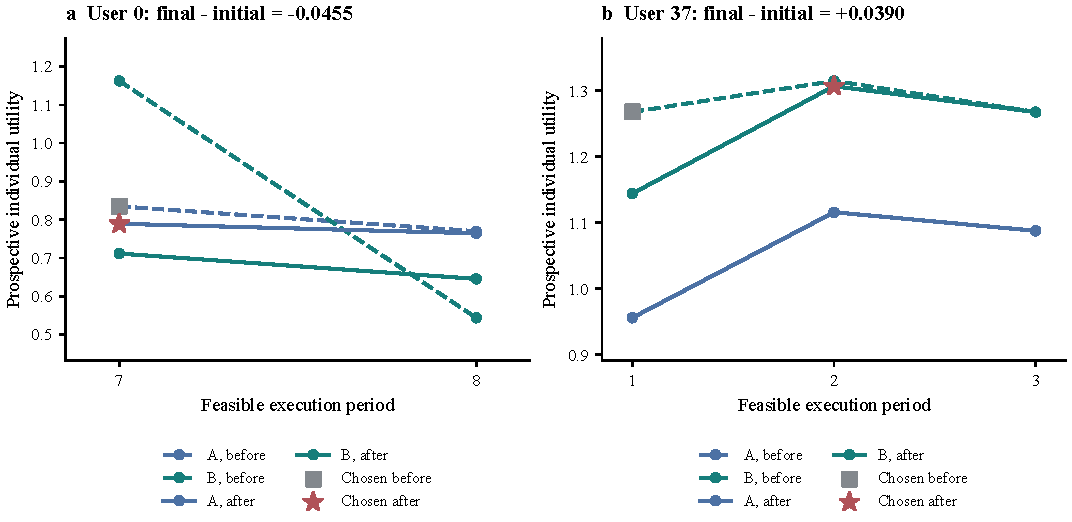
\includegraphics[width=\textwidth]{individual_time_choices.pdf}
\caption{Individual prospective utility over every feasible period and both manufacturers. Dashed curves use the initial load state; solid curves use the final state. Each candidate includes the focal agent's own contribution at its prospective destination. Squares and stars mark the chosen initial and final actions. User 0 is the predeclared example; user 37 is the explicitly post-hoc time-movement example. Only the latter changes time. Both have zero profitable final unilateral deviation, despite different before--after utility signs. These curves refer to one realized price pair, not the mixed-strategy averages in Table~\ref{tab:main}.}
\label{fig:users}
\end{figure}

\subsection{TOU does not outperform the strategic uniform-price benchmark}
When both regimes are allowed to reach their own manufacturer and user equilibria, the conclusion changes. TOU reduces mean utility from 1.1009 to 0.9772, an absolute loss of 0.1237. Mean bills increase by 13.66\%, generalized costs increase by 13.76\%, and expected peak load rises from 52.39 to 53.06 (1.29\%). Only 43 agents (17.92\%) have higher expected utility, while 197 (82.08\%) have lower expected utility.

\begin{figure}[htbp]
\centering
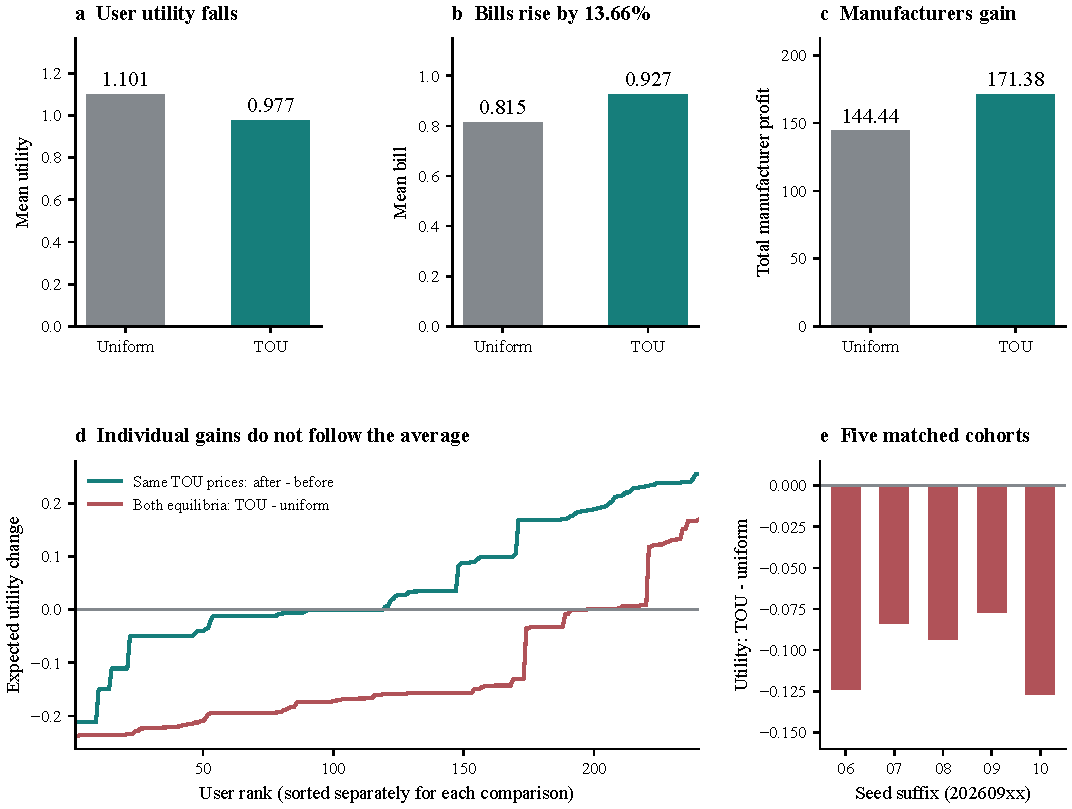
\includegraphics[width=\textwidth]{fair_tariff_comparison.pdf}
\caption{Tariff comparison with manufacturer competition and user Nash responses in both regimes. (a--c) Mean utility and bills, and total manufacturer profit. (d) All 240 expected utility changes, sorted separately within each comparison; the horizontal ranks do not identify the same user across curves. (e) Paired TOU-minus-uniform mean utility differences for all five predefined cohorts. There is no user-welfare improvement over the strategic uniform benchmark in these cohorts. Exact finite-mixture expectations are shown without statistical error bars.}
\label{fig:tariffs}
\end{figure}

Manufacturer A profit rises from 94.10 to 108.82, and B profit rises from 50.34 to 62.56. Total manufacturer profit increases by 26.94 units. The model has conserved demand, no participation constraint, and no user exit, so a richer price menu can benefit manufacturers without preserving user utility. This is a result about the declared model. It does not establish a general theorem that TOU harms users, just as the same-price adaptation gain does not establish general TOU superiority.

\subsection{Convergence, resource outcomes, and finite-game checks}
The representative TOU price pair requires 96 strict moves and six full sweeps, the last with no moves. Its exact potential decreases from 255.6964 to 238.8664, and maximum user regret falls from 0.6001 to zero. Mean utility is not monotone along the path (Fig.~\ref{fig:convergence}), consistent with the externalities in the potential proof. Figure~\ref{fig:resource} shows that the aggregate peak change also redistributes manufacturer congestion across periods.

\begin{figure}[htbp]
\centering
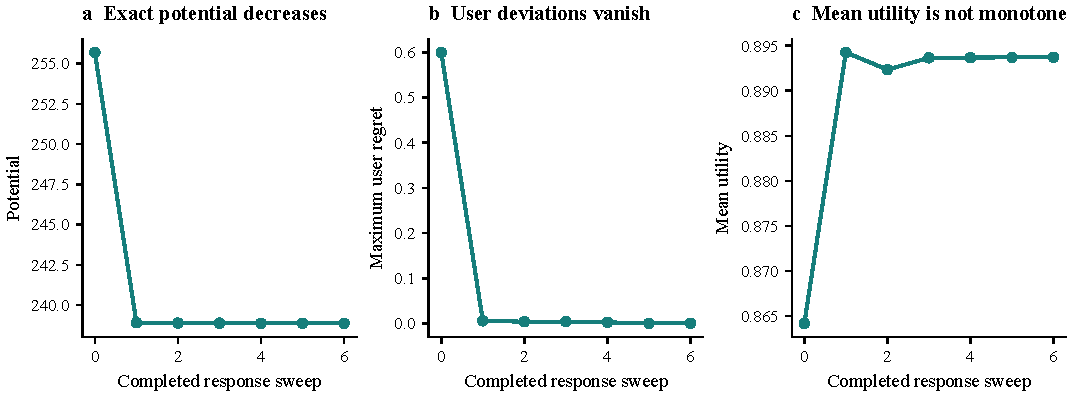
\includegraphics[width=\textwidth]{user_convergence.pdf}
\caption{Unsmoothened sweep-level results at the representative price pair. The exact potential decreases, user deviations vanish, and average utility need not increase in every sweep. These are one-price-pair values; they are not the support-weighted values in Fig.~\ref{fig:beforeafter}.}
\label{fig:convergence}
\end{figure}

The main uniform equilibrium has manufacturer support sizes 3/3; TOU has 4/4. Every declared price pair, including those outside support, has a certified user response. We replayed 5,625 distinct price pairs for each of nine scenario--cohort configurations, totaling 50,625 pairs. The nested menus and fixed-mean control are subsets of the baseline replay. Independently recomputed manufacturer matrices have zero maximum discrepancy from the recorded matrices. The largest metric discrepancy is $2.22\times10^{-16}$ and the largest full-menu manufacturer regret is $4.27\times10^{-14}$; independently computed user regret is zero throughout. A separate brute-force check rebuilt complete assignments for all 824 feasible unilateral user alternatives at the representative equilibrium, again with zero positive regret. These checks use the same selected assignment solver but separate direct utility, accounting, and deviation formulas; they are not an independent equilibrium-selection algorithm.

\begin{figure}[htbp]
\centering
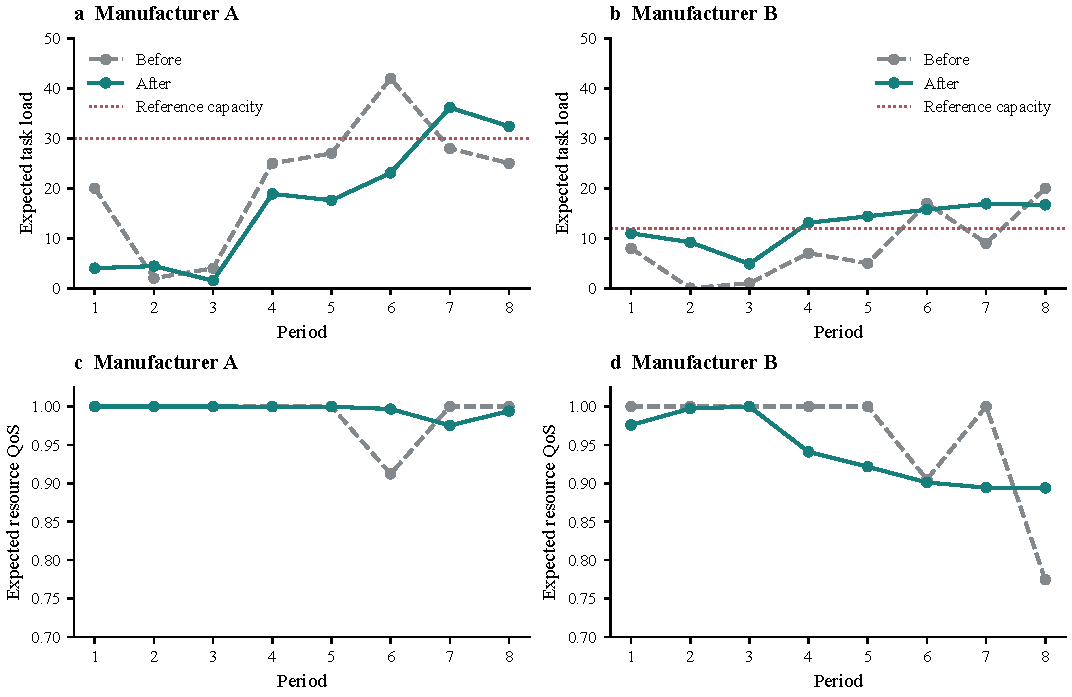
\includegraphics[width=\textwidth]{provider_load_quality.pdf}
\caption{Manufacturer-level before--after outcomes at the same final TOU prices. Top: expected task counts and reference capacities, with common vertical scales. Bottom: expected resource QoS, also on common scales. Resource QoS weights each price realization, whereas mean user QoS additionally weights the tasks assigned to that resource. A lower total peak does not imply improvement of every resource's QoS.}
\label{fig:resource}
\end{figure}

\subsection{Menu refinement, boundary cases, and the mean-price control}
Table~\ref{tab:menus} shows meaningful discretization effects. A TOU equilibrium on the coarsest menu leaves B a 13.5894-unit profitable deviation on the final menu; on the middle menu the corresponding gain is 2.1010. The final menu passes the declared finite test, but this does not show that nine axis points approximate a continuous equilibrium adequately. In particular, a visually stable utility curve across a few grids would not substitute for a continuous-domain check.

\begin{table}[htbp]
\centering
\caption{Nested menu comparison. The last two columns re-evaluate the TOU equilibrium against all final-menu manufacturer actions. For the final row, they are its own full-menu regrets.}
\label{tab:menus}
\small
\begin{tabular}{@{}rrrrrr@{}}
\toprule
Axis points & Rules U/TOU & Utility U & Utility TOU & A regret & B regret \\
\midrule
\inputtable{artifacts/user_provider_game/20260906/menu_table.tex}
\bottomrule
\end{tabular}
\end{table}

All four predefined boundary cases retain a negative TOU-minus-uniform utility difference (Table~\ref{tab:boundary}). With no time flexibility, provider substitution remains available but no user can defer. The adverse tariff effect therefore cannot be interpreted solely as a delay burden. The five cohort differences range from $-0.1271$ to $-0.0770$, averaging $-0.1011$. They assess variation across synthetic instances, not a real-market confidence interval.

\begin{table}[htbp]
\centering
\caption{Predefined boundary cases and additional cohorts, all on the final menu. U denotes uniform pricing. Each row compares the same underlying users across both regimes.}
\label{tab:boundary}
\small
\begin{tabular}{@{}lrrrrr@{}}
\toprule
Case & Utility U & Utility TOU & Difference & Peak U & Peak TOU \\
\midrule
\inputtable{artifacts/user_provider_game/20260906/boundary_table.tex}
\bottomrule
\end{tabular}
\end{table}

Fixing each manufacturer's unweighted mean price at 0.75 does not resolve user protection. The fixed uniform schedule yields mean utility 1.2330, mean bill 0.7500, and peak 51.00. Allowing slope competition at exactly the same mean yields utility 1.1857, bill 0.7879, and peak 48.80. This control reduces the peak while increasing actual bills. An unweighted mean-price constraint is not a demand-weighted payment constraint.

We also change the response order to natural, reverse, and independently permuted user indices at the baseline TOU support prices. All three produce user equilibria, with mean utility between 0.97749 and 0.97792, compared with 0.97718 under the declared order. This is a limited support-price selection check. We do not claim a manufacturer equilibrium under any changed response rule, because its complete off-support payoff matrices were not re-solved.

\FloatBarrier
\section{Discussion and Limitations}
The requested user objective is explicit in Eq.~(\ref{eq:utility}), and every final user chooses an individually optimal feasible provider--time action up to tolerance. Nevertheless, ``the algorithm makes users individually stable'' is weaker than ``the pricing mechanism improves every user's outcome.'' The same-price experiment supports average adaptation benefits; the matched tariff experiment rejects average user-welfare superiority for this calibration. The manufacturer's profit objective does not contain a user compensation or participation term.

A welfare-oriented extension would need an additional mechanism, such as an opt-out uniform contract, a participation constraint relative to a declared baseline, or funded rebates. Such an extension would change the action sets or payment game and require new equilibrium calculations. Simply relabeling the present profit game as user-welfare optimization, changing parameters until a positive figure appears, or enforcing an unweighted mean tariff is not a substitute. We have not implemented or validated those extensions.

The present theoretical guarantee depends on unit workloads and a common congestion function. Real requests have heterogeneous token lengths, model preferences, privacy constraints, and variable delay sensitivity. The capacity curve is a transferable proxy, not a queueing model or calibrated response surface for every service. Future work should test heterogeneous loads, participation, and uncertain arrivals without assuming that the current exact potential survives. User preferences and timing costs need behavioral data; BurstGPT alone cannot identify them.

Manufacturers commit before user choices, and the response order is a declared equilibrium-selection convention. The model does not establish convergence of simultaneous online learning by manufacturers and users. Equilibrium uniqueness is not claimed at either layer. The manufacturer's certificate is restricted to 75 declared TOU rules, with visible coarse-menu sensitivity. A direct-access two-manufacturer result does not validate an intermediary or routing policy. These boundaries remain even though all finite numerical checks pass.

\section{Conclusion}
An explicit atomic user game makes it possible to verify both the user's timing decision and the manufacturer's pricing incentives. At the same final TOU prices, autonomous best responses give a clear measured before--after improvement in average bills, generalized costs, and peak load. Full unilateral-deviation checks certify individual stability, but congestion externalities leave some users worse off. With equally strategic users in both tariff regimes, the computed TOU equilibrium raises bills and lowers mean user utility relative to the uniform equilibrium in all five predefined cohorts. The distinction between adaptation and tariff welfare is therefore central to interpreting the algorithm, not a secondary qualification.

\appendix
\section{Price Support and Reproducibility}
Table~\ref{tab:support} lists every active final-menu tariff. Manufacturers randomize independently; joint weights are products of the two marginal probabilities. Rule identifiers are zero-based artifact indices. All inactive rules and both full payoff matrices remain in the experiment record, so the support table is not the deviation set.

\begin{table}[H]
\centering
\caption{Active manufacturer strategies on the final menu. All unlisted rules have zero reported probability.}
\label{tab:support}
\begin{tabular}{@{}llrrrr@{}}
\toprule
Regime & Manufacturer & Rule ID & Mean $\beta$ & Slope $\alpha$ & Probability \\
\midrule
\inputtable{artifacts/user_provider_game/20260906/price_support_table.tex}
\bottomrule
\end{tabular}
\end{table}

The accompanying package contains the complete experiment, all 240 user outcome rows, period outcomes, convergence traces, boundary comparisons, exact menu matrices, figure source data, code and input hashes, and the independent replay certificate. The experiment uses Python 3.12.13, NumPy 2.4.4, and SciPy 1.17.1 in its recorded run. Four-process execution limits native BLAS threads to one per worker. The protocol, core solver, manufacturer solver, data profile, and quality calibration are pinned by SHA-256. The figure and bundle manifests additionally bind the reporting code, vector exports, manuscript, and PDF. The short experiment identifier is \texttt{3e7f8993088822f32}.

The data are synthetic individual agents with empirical workload-shape and quality anchors. No new human-subject or live pricing experiment is claimed. The scientific certificate is limited to the stated finite model; numerical verification is not empirical validation or a submission-readiness declaration.

\clearpage
\bibliographystyle{plainnat}
\bibliography{verified_refs}
\end{document}
